\chapter{Marco Teórico y Tecnológico}
\label{chap:marco_teorico}

Este capítulo presenta los fundamentos teóricos, legales y tecnológicos que sustentan la solución implementada: el marco criptográfico y normativo aplicable a la firma electrónica en la Argentina, y las capas de virtualización, orquestación y almacenamiento sobre las que se apoya el despliegue.

\section{Modelos de Despliegue: \textit{On-Premise} y \textit{Self-Hosted}}
\label{sec:onpremise_selfhosted}

Para la implementación de Documenso se adoptó una estrategia que combina los modelos \textit{on-premise} y \textit{self-hosted}. Aunque la industria suele emplear ambos términos de manera intercambiable, en este trabajo se utilizan con alcances distintos.

El carácter \textit{on-premise} responde a que el software opera sobre hardware alojado físicamente en la facultad ---clústeres de virtualización Proxmox y servidores TrueNAS ya disponibles---, lo que evita los costos recurrentes de una infraestructura en la nube (IaaS). La condición \textit{self-hosted} implica que la propia institución aprovisiona, configura y mantiene la plataforma, en lugar de delegar esas responsabilidades a un proveedor de \textit{Software as a Service} (SaaS). En conjunto, el modelo otorga control completo sobre las configuraciones del sistema, la arquitectura de red, las políticas de retención y el ciclo de vida de los documentos, a cambio de asumir la carga operativa del mantenimiento.

\subsection{Software de Código Abierto y Licencia AGPL-3.0}

Documenso se distribuye en su Community Edition bajo licencia AGPL-3.0 e incluye las funcionalidades centrales de firma documental y autoalojamiento \cite{documenso_community,documenso_github}. La AGPL-3.0 conserva las libertades habituales de la familia GPL ---uso, estudio, modificación, distribución--- y agrega la obligación de publicar las modificaciones también cuando el software se ofrece como servicio a través de una red \cite{documenso_community,agpl_fossa,agpl_ultralytics}.

Para este trabajo, la Community Edition resultó adecuada porque habilitó el despliegue sobre infraestructura propia, la revisión del comportamiento interno de la plataforma y la adaptación de la solución sin depender de una licencia comercial. La documentación de Documenso señala que las funciones empresariales y la posibilidad de mantener modificaciones privadas corresponden a la Enterprise Edition \cite{documenso_community}.

\section{Fundamentos de Seguridad de la Información}
\label{sec:fundamentos_seguridad}

El diseño de la plataforma se enmarca en la arquitectura de seguridad OSI X.800 \cite{saade_redes_2024}. Los servicios relevantes para un sistema de gestión documental sobre infraestructura institucional son: confidencialidad, integridad, disponibilidad, autenticación, control de acceso y no repudio.

La solución implementada materializa cada servicio mediante componentes concretos del \textit{stack}: la autenticación se delega en Google OAuth~2.0 con cuentas institucionales; el control de acceso opera bajo un modelo Role-Based Access Control (RBAC) dentro de Documenso; la integridad y el no repudio se sustentan en el sellado criptográfico del documento; la confidencialidad se resguarda mediante cifrado TLS en tránsito y restricción del acceso al dominio institucional; y la disponibilidad se apoya en la redundancia RAID~6, los respaldos automatizados hacia MinIO y la separación entre cómputo y almacenamiento.

\section{Mecanismos Técnicos de Firma Digital}
\label{sec:mecanismo_tecnico}

La implementación de los servicios de integridad y no repudio se basa en criptografía de clave pública. Este esquema utiliza un par de claves vinculadas matemáticamente: una clave privada ($KR$), de conocimiento exclusivo de su propietario, y una clave pública ($KU$), distribuida libremente para verificación.

\subsection{Proceso de Generación de Firma}
El flujo técnico empleado por Documenso \cite{documenso_docs_signing} para sellar un documento consiste en calcular un \textit{hash} criptográfico del contenido, cifrarlo con la clave privada ($KR$) asociada al certificado de la plataforma e incrustar la firma resultante en la estructura del archivo PDF. La Figura~\ref{fig:proceso_firma} ilustra el procedimiento general de generación y verificación de firma digital.

\begin{figure}[H]
    \centering
    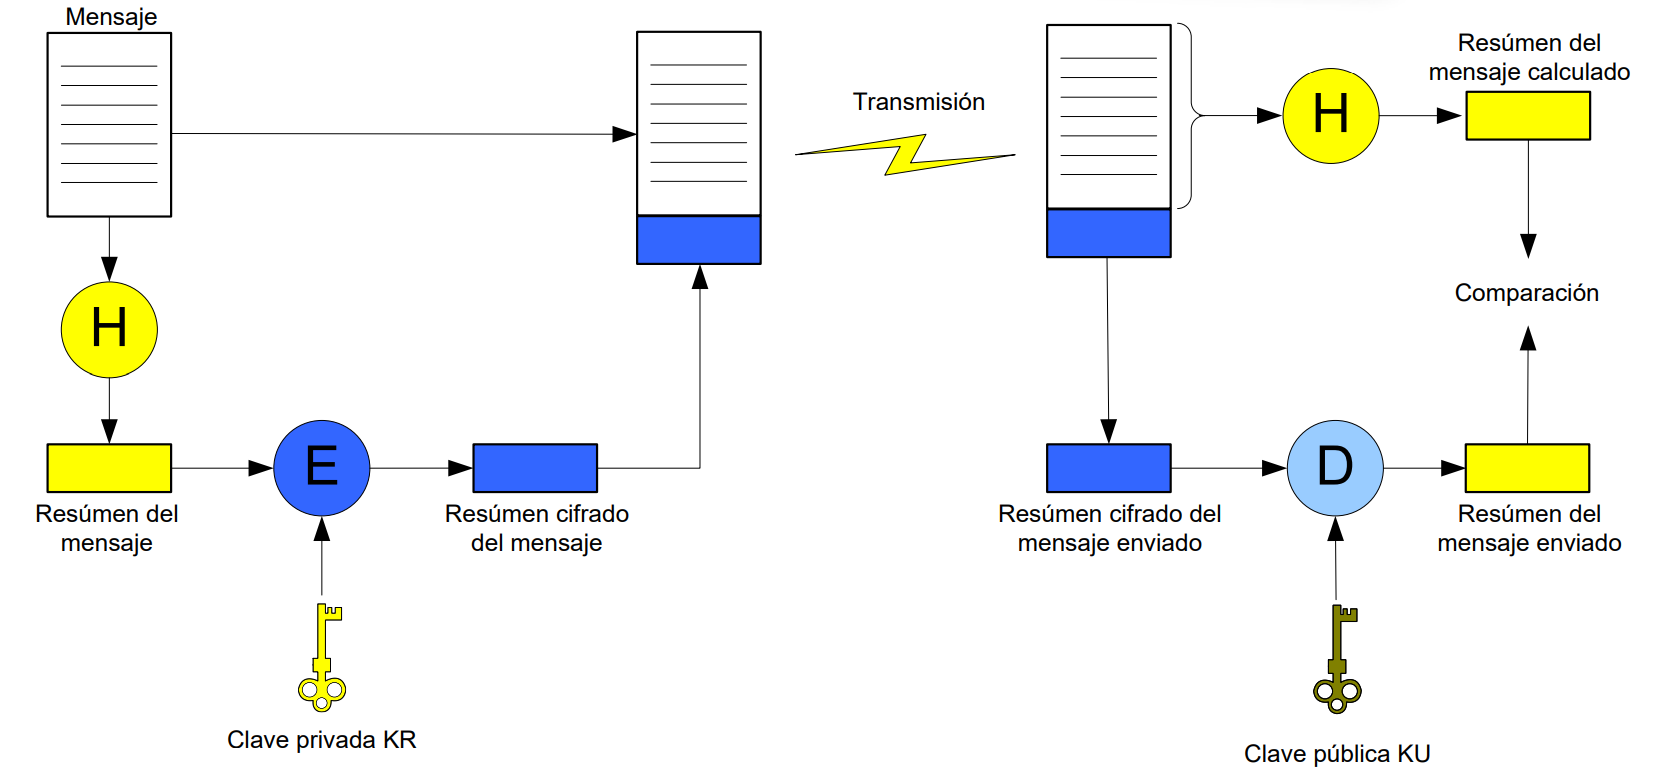
\includegraphics[width=0.8\textwidth]{figuras/capitulo2/ProcesodeFirma.png}
    \caption[Proceso de generación de firma]{Proceso de generación y verificación de firma digital. Extraído de \cite{saade_redes_2024}.}
    \label{fig:proceso_firma}
\end{figure}

La firma se aplica a nivel de plataforma y no por cada firmante individual. Las acciones de cada usuario ---trazos de firma, textos, casillas de verificación--- quedan registradas en el sistema; una vez que todos los participantes completan su intervención, el documento se sella criptográficamente bajo el certificado de la instancia institucional. Este sellado proporciona dos garantías: integridad ---el documento no fue alterado desde el momento de la firma--- y autenticidad ---el PDF fue firmado por el titular del certificado---. Si el archivo se modifica con posterioridad, la firma deja de ser válida y los lectores PDF advierten sobre la alteración \cite{documenso_docs_signing}.

\subsection{Certificados de Clave Pública y CA Interna}
Debido a que la $KU$ es de acceso general, se emplean certificados digitales que vinculan la clave con su titular mediante la firma de una Autoridad de Certificación (CA).

En esta implementación se utiliza un certificado autofirmado generado dentro del entorno institucional. La documentación de Documenso distingue entre confianza del certificado y validez criptográfica de la firma \cite{documenso_docs_signing,documenso_docs_cert_config}: al no pertenecer a una cadena de confianza comercial, los lectores PDF pueden advertir que el emisor no fue validado por una tercera parte, pero esa condición no invalida la integridad criptográfica del documento ni impide su uso en circuitos administrativos internos.

En este trabajo, el material criptográfico se administró como un contenedor PKCS\#12 codificado en Base64 e inyectado mediante variables de entorno, tal como se documenta en el Apéndice~\ref{AppendixB:Crypto}. La restricción legal depende del certificado y no de la plataforma: Documenso soporta certificados X.509 emitidos por autoridades certificantes licenciadas \cite{documenso_docs_cert_config}, de modo que el certificado local podría reemplazarse sin modificar la infraestructura base si la institución requiriera validación ante terceros.

\section{Marco Legal Argentino: Ley 25.506}
\label{sec:marco_legal}

La validez jurídica de la solución se encuadra en la Ley 25.506 de Firma Digital \cite{ley25506}, que establece una distinción fundamental:

\begin{itemize}
    \item Firma Digital (Art. 2 y Art. 9): el Artículo 2 define a la firma digital como el resultado de aplicar a un documento digital un procedimiento matemático que requiere información de exclusivo conocimiento del firmante, bajo su absoluto control. La verificación debe permitir identificar al firmante y detectar cualquier alteración del documento posterior a la firma. El Artículo 9 exige, entre otros requisitos, que el certificado haya sido emitido o reconocido por un certificador licenciado.
    \item Firma Electrónica (Art. 5): se entiende por firma electrónica al conjunto de datos electrónicos integrados, ligados o asociados de manera lógica a otros datos electrónicos, utilizado por el signatario como medio de identificación, que carezca de alguno de los requisitos legales para ser considerada firma digital. En caso de ser desconocida, corresponde a quien la invoca acreditar su validez.
\end{itemize}

Dado que el sistema utiliza una Autoridad Certificante propia sin licencia estatal ---lo que incumple el requisito del Art. 9---, la solución se clasifica legalmente como firma electrónica. Su validez administrativa es, no obstante, plena dentro del ámbito interno de la organización, con fundamento en el acuerdo entre las partes y en la trazabilidad técnica que proporciona la plataforma.

\section{Infraestructura de Virtualización y Despliegue}
\label{sec:infraestructura}

La arquitectura del despliegue se organizó en capas para desacoplar los servicios de la administración directa del hardware y simplificar las tareas de operación y recuperación.

\subsection{Plataforma de Virtualización y Orquestación}

La infraestructura de cómputo se estructura en tres niveles. En la base, Proxmox VE \cite{proxmox_docs,bilbao_lutz_virtualizacion_2024} administra los recursos físicos del servidor y aloja un contenedor LXC. Se optó por LXC en lugar de una máquina virtual KVM porque comparte el kernel del anfitrión, lo que reduce la sobrecarga de CPU y memoria ---condición relevante dado el procesador Xeon E5620 disponible---.

Dentro de ese contenedor se ejecuta Docker \cite{docker_docs} y, sobre él, opera Coolify \cite{coolify_docs}: una PaaS autoalojable de código abierto que centraliza la gestión de despliegues, variables de entorno, dominios y respaldos en un panel web unificado, sin ceder el control de la infraestructura a un proveedor externo. Este conjunto ---LXC, Docker y Coolify--- ya se encontraba aprovisionado por el área de sistemas de la FACET como nodo de orquestación base de la facultad.

El aporte de este trabajo consistió en desplegar el sistema de firmas sobre esa plataforma preexistente. Documenso distribuye su \textit{stack} como un conjunto de servicios definidos en un archivo \texttt{docker-compose.yml} \cite{documenso_github}, lo que exige un entorno contenerizado con Docker como requisito mínimo. La justificación de la adopción de Coolify y los detalles de configuración se desarrollan en el Capítulo~\ref{chap:diseno_implementacion}.

\subsection{\textit{Reverse Proxy} y Enrutamiento Dinámico (Traefik)}
Traefik actúa como \textit{reverse proxy} dentro de la red de contenedores, enrutando dinámicamente el tráfico entrante (HTTP/HTTPS) hacia los contenedores internos correspondientes según las reglas de dominio declaradas \cite{traefik_docs}. Este desacoplamiento entre la dirección pública del servicio y su ubicación real dentro de la infraestructura permite publicar múltiples aplicaciones desde un único punto de entrada.

\section{Arquitectura de Almacenamiento de Objetos}
\label{sec:almacenamiento}

La persistencia de los documentos digitales se resuelve mediante una arquitectura que separa la gestión física de los discos del acceso lógico a los archivos. Esta capa se vincula directamente con la disponibilidad definida en la Sección~\ref{sec:fundamentos_seguridad}, ya que de ella depende que los documentos permanezcan accesibles cuando se los requiere. Se utiliza TrueNAS Community Edition \cite{truenas} como plataforma de almacenamiento base y MinIO \cite{minio} como motor de objetos compatible con el protocolo S3.

\subsection{Gestión Física y Resiliencia (TrueNAS y ZFS)}
\label{subsec:teoria_raid}

TrueNAS Community Edition \cite{truenas} gestiona la capa física mediante ZFS sobre un arreglo RAID~6 \cite{techtarget_raid6}. Esta combinación proporciona resiliencia ante fallas de disco y mitiga la degradación silenciosa de datos (\textit{bit-rot}). No obstante, la redundancia de hardware no sustituye una política de respaldos lógicos: protege frente a fallas físicas, pero no frente a errores de software, eliminaciones accidentales o manipulación indebida de los datos \cite{techtarget_raid6,techtarget_retention}.

\subsection{MinIO: Almacenamiento de Objetos S3}
Sobre la infraestructura de TrueNAS se utiliza MinIO para la gestión de los documentos mediante el protocolo S3. Este componente es clave en el diseño por dos motivos:

\begin{itemize}
    \item Separación entre aplicación y almacenamiento: Documenso guarda y recupera documentos a través de una interfaz S3 sin depender de carpetas locales del servidor de aplicación. Esto permite trasladar o ampliar el almacenamiento sin modificar la lógica del sistema y habilita, a futuro, esquemas de respaldo híbrido entre infraestructura local y servicios externos compatibles.
    \item Retención e inmutabilidad: mediante Object Lock, MinIO aplica políticas de conservación que impiden la modificación o eliminación prematura de los documentos almacenados \cite{minio_object_locking}. Para los documentos firmados, esta capacidad preserva evidencia de que el archivo no fue alterado después de su incorporación al repositorio.
\end{itemize}

Mientras ZFS se ocupa de la redundancia y la integridad física en los discos, MinIO proporciona el control necesario para garantizar la persistencia e inmutabilidad de los archivos firmados a nivel de software.

\subsection{Principios de Respaldo y Retención de Datos}
\label{subsec:respaldo_retencion}

Un despliegue \textit{on-premise} exige que la institución asuma la responsabilidad completa sobre la preservación de los datos, dado que no existe un proveedor externo que gestione copias de seguridad o garantice la recuperación ante desastres \cite{techtarget_retention}. Una política de respaldo define qué información debe copiarse, con qué frecuencia, dónde se conserva y bajo qué procedimiento puede recuperarse. Una política de retención establece durante cuánto tiempo se mantienen esas copias y en qué momento pueden eliminarse de acuerdo con criterios operativos, normativos o de capacidad \cite{techtarget_retention,pgbarman_retention}.

En una plataforma documental, ambas políticas deben contemplar al menos dos dominios con necesidades distintas:

\begin{itemize}
    \item Datos transaccionales: usuarios, permisos, estados de firma y registros de auditoría. Su pérdida comprometería la trazabilidad operativa del sistema.
    \item Repositorio documental: archivos cargados y sus versiones firmadas, cuya preservación requiere reglas claras de conservación e inmutabilidad.
\end{itemize}

La implementación concreta de estas políticas ---frecuencias de ejecución, períodos de retención y procedimientos de restauración--- se documenta en el Capítulo~\ref{chap:diseno_implementacion}.

\section{Gestión de Identidad y Autorización: Google OAuth 2.0}
\label{sec:identidad}

El control de acceso a la plataforma se delega en Google Workspace mediante el protocolo OAuth 2.0 \cite{oauth2}. Esto desacopla la autenticación de la lógica de la aplicación y evita que el servidor local almacene credenciales. El flujo de redirección e intercambio de tokens asegura que Documenso solo reciba la información estrictamente necesaria para validar la identidad institucional del usuario.

Para completar la integración se registra la instancia en Google Cloud y se obtiene un Client ID y un Client Secret. El detalle de las variables de entorno y los parámetros concretos de configuración se presenta en el Apéndice~\ref{AppendixB}.


